% !TEX TS-program = pdflatex
% !TEX encoding = UTF-8 Unicode

% This is a simple template for a LaTeX document using the "article" class.
% See "book", "report", "letter" for other types of document.

\documentclass[11pt]{article} % use larger type; default would be 10pt

\usepackage[utf8]{inputenc} % set input encoding (not needed with XeLaTeX)

%%% Examples of Article customizations
% These packages are optional, depending whether you want the features they provide.
% See the LaTeX Companion or other references for full information.

%%% PAGE DIMENSIONS
\usepackage{geometry} % to change the page dimensions
\geometry{a4paper} % or letterpaper (US) or a5paper or....
% \geometry{margin=2in} % for example, change the margins to 2 inches all round
% \geometry{landscape} % set up the page for landscape
%   read geometry.pdf for detailed page layout information
\usepackage[font=small]{caption}
\usepackage{graphicx} % support the \includegraphics command and options

% \usepackage[parfill]{parskip} % Activate to begin paragraphs with an empty line rather than an indent

%%% PACKAGES
\usepackage{booktabs} % for much better looking tables
\usepackage{array} % for better arrays (eg matrices) in maths
\usepackage{paralist} % very flexible & customisable lists (eg. enumerate/itemize, etc.)
\usepackage{verbatim} % adds environment for commenting out blocks of text & for better verbatim
\usepackage{subfig} % make it possible to include more than one captioned figure/table in a single float
\usepackage{changes} % for subscript

% These packages are all incorporated in the memoir class to one degree or another...

%%% HEADERS & FOOTERS
\usepackage{fancyhdr} % This should be set AFTER setting up the page geometry
\pagestyle{fancy} % options: empty , plain , fancy
\renewcommand{\headrulewidth}{0pt} % customise the layout...
\lhead{}\chead{}\rhead{}
\lfoot{}\cfoot{\thepage}\rfoot{}

%%% SECTION TITLE APPEARANCE
\usepackage{sectsty}
\allsectionsfont{\sffamily\mdseries\upshape} % (See the fntguide.pdf for font help)
% (This matches ConTeXt defaults)

%%% ToC (table of contents) APPEARANCE
\usepackage[nottoc,notlof,notlot]{tocbibind} % Put the bibliography in the ToC
\usepackage[titles,subfigure]{tocloft} % Alter the style of the Table of Contents
\renewcommand{\cftsecfont}{\rmfamily\mdseries\upshape}
\renewcommand{\cftsecpagefont}{\rmfamily\mdseries\upshape} % No bold!

%%% END Article customizations

\usepackage{listings}
\usepackage{color}
\lstset{language=C++} 
\definecolor{mygreen}{rgb}{0,0.6,0}
\definecolor{mygray}{rgb}{0.5,0.5,0.5}
\definecolor{mymauve}{rgb}{0.58,0,0.82}


\lstset{ %
  backgroundcolor=\color{white},   % choose the background color; you must add \usepackage{color} or \usepackage{xcolor}
  basicstyle=\footnotesize,        % the size of the fonts that are used for the code
  breakatwhitespace=false,         % sets if automatic breaks should only happen at whitespace
  breaklines=true,                 % sets automatic line breaking
  captionpos=b,                    % sets the caption-position to bottom
  commentstyle=\color{mygreen},    % comment style
  deletekeywords={...},            % if you want to delete keywords from the given language
  escapeinside={\%*}{*)},          % if you want to add LaTeX within your code
  extendedchars=true,              % lets you use non-ASCII characters; for 8-bits encodings only, does not work with UTF-8
  frame=single,	                   % adds a frame around the code
  keepspaces=true,                 % keeps spaces in text, useful for keeping indentation of code (possibly needs columns=flexible)
  keywordstyle=\color{blue},       % keyword style
  language=C,                 % the language of the code
  otherkeywords={*,...},           % if you want to add more keywords to the set
  numbers=left,                    % where to put the line-numbers; possible values are (none, left, right)
  numbersep=5pt,                   % how far the line-numbers are from the code
  numberstyle=\tiny\color{mygray}, % the style that is used for the line-numbers
  rulecolor=\color{black},         % if not set, the frame-color may be changed on line-breaks within not-black text (e.g. comments (green here))
  showspaces=false,                % show spaces everywhere adding particular underscores; it overrides 'showstringspaces'
  showstringspaces=false,          % underline spaces within strings only
  showtabs=false,                  % show tabs within strings adding particular underscores
  stepnumber=2,                    % the step between two line-numbers. If it's 1, each line will be numbered
  stringstyle=\color{mymauve},     % string literal style
  tabsize=2,	                   % sets default tabsize to 2 spaces
  title=\lstname                   % show the filename of files included with \lstinputlisting; also try caption instead of title
}

%%% The "real" document content comes below...

\title{NS2 Application for Video traffic}
\author{Saba Ahsan}
%\date{} % Activate to display a given date or no date (if empty),
         % otherwise the current date is printed 

\begin{document}
\maketitle

\section{Introduction}
This document describes the Video traffic Application (VmApp) for Ns-2 in brief. It includes the instructions on how to compile the code and a few examples to show its usage.

\section{What it does}

VmApp generates video traffic using a media file and a target file. Both files consist of media bitrate values for every second. The media files are included in the git package in the folder ns2-videosrc/samplefiles/. Each media file has 7 columns (0 - 6), but VmApp only uses three of them: column 2 is the number of bytes, column 3 is the instantaneous bit rate in kbps and  column 6 is the timestamp in milliseconds. The cumulative bit rate of the sample stream is calculated in the beginning by summing all the values in column 2 and dividing by the last timestamp in column 6. This is then used for calculating the sending bit rate R\textsubscript{achieve} as follows 


\begin{equation}
R_{achieve}= \frac{R_{media}}{R_{cumulative}} \times R_{target}
\end{equation}
\begin{figure}[!ht]
  \centering
    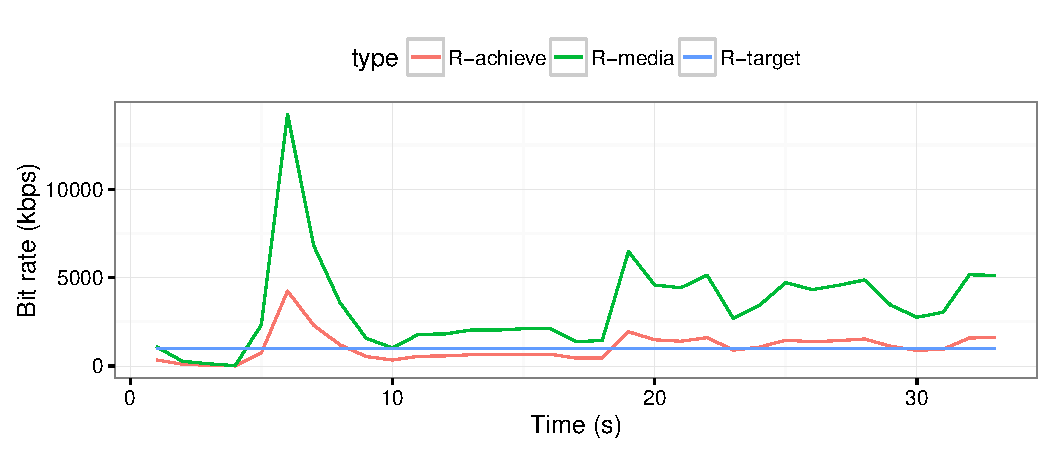
\includegraphics[width=0.8\textwidth]{docfiles/rates.pdf}
  \caption{A comparison of the media and achieved rate when 1000kbps target rate was used.}
\end{figure}

This value is calculated per second, reading R\textsubscript{media} and R\textsubscript{target} from the respective files. The frame rate is defined by the user (if not the default value is used). Based on R\textsubscript{achieve} and the frame rate, VmApp can then calculate the size of each frame (all frames are of the same size during that second).  




\section{How to build}

\begin{enumerate}
	\item Place the "vdo" directory  (containing vm-udp.cc, vm-udp.h, vm-app.cc and vm-app.h) in the ns-2.35 folder\footnote{http://www.isi.edu/nsnam/ns/ns-build.html}. 

	\item In “common/packet.h” define PT\_Multimedia and change PT\_NTYPE to 74. Furthermore, add PT\_Multimedia to p\_info class. 

\begin{lstlisting}[title="packet.h"]
        // insert new packet types here

static packet_t       PT_Multimedia = 73; //The new PT for MM
static packet_t       PT_NTYPE = 74; // This MUST be the LAST one
\end{lstlisting}

\begin{lstlisting}[title="packet.h"]
        static bool data_packet(packet_t type) {
                return ( (type) == PT_TCP || \
                         (type) == PT_TELNET || \
                         (type) == PT_CBR || \
                         (type) == PT_AUDIO || \
                         (type) == PT_VIDEO || \
                         (type) == PT_ACK || \
                         (type) == PT_SCTP || \
                         (type) == PT_SCTP_APP1 || \
                         (type) == PT_Multimedia || \
                         (type) == PT_HDLC \
                        );
        }
        static packetClass classify(packet_t type) {            
                if (type == PT_DSR || 
                    type == PT_MESSAGE || 
                    type == PT_TORA ||
                    type == PT_PUMA ||
                    type == PT_AODV ||
                    type == PT_MDART)
                        return ROUTING;         
                if (type == PT_TCP || 
                    type == PT_TELNET || 
                    type == PT_CBR || 
                    type == PT_AUDIO || 
                    type == PT_VIDEO || 
                    type == PT_ACK || 
                    type == PT_SCTP || 
                    type == PT_SCTP_APP1 || 
                    type == PT_Multimedia || 
                    type == PT_HDLC)
                        return DATApkt;
\end{lstlisting}


	\item In “tcl/lib/ns-packet.tcl” register the new application header
\begin{lstlisting}[title="ns-packet.tcl"]
# Other:
        Encap   # common/encap.cc
        IPinIP  # IP encapsulation 
        HDLC    # High Level Data Link Control
        Multimedia #Self define MM
\end{lstlisting}

	\item In “Agent” class in “common/agent.h” add supportVM() and enableVM()
\begin{lstlisting}[title="agent.h"]
        inline packet_t get_pkttype() { return type_; }

        //add supportvm MM
        virtual int supportVM() { return 0; }
        virtual void enableVM() {}

\end{lstlisting}

	\item In “Application” class in “apps/app.h” add recv\_msg() method
\begin{lstlisting}[title="app.h"]
class Agent;

class Application : public Process {
public:
        Application();
        virtual void send(int nbytes);
        virtual void recv(int nbytes);
        virtual void resume();

        //vmap recv_msg MM
        virtual void recv_msg(int nbytes, const char * msg=0){};
\end{lstlisting}

	\item Add default values for new parameters at the end of “tcl/lib/ns-default.tcl”. 

\begin{lstlisting}[title="ns-default.tcl"]

Application/VmApp set pktsize_ 1000
Application/VmApp set target_rate_ 1000

\end{lstlisting}

	\item In “Makefile.in” add “vm-app.o” and “vm-upd.o” and run “./configure”/. Run “Make clean ” and then re-compile NS type “make”.
\begin{lstlisting}[title="Makefile"]
        wpan/p802_15_4trace.o wpan/p802_15_4transac.o \
        apps/pbc.o \
        vdo/vm-app.o \
        vdo/vm-udp.o \
        $(OBJ_STL)


\end{lstlisting}

\end{enumerate}
\section{Examples}

\end{document}
